% \documentclass[11pt,twoside,a4paper]{article}
% \usepackage{times}

% \usepackage{xeCJK}

% \setmainfont{Times New Roman}

% \setCJKmainfont{Songti SC}
\documentclass[10pt]{ctexart}
% \usepackage[UTF-8]{ctex}
\usepackage{amsmath}
\usepackage{amssymb}  %为了能使用\mathbb{H} 
\usepackage{booktabs}
\usepackage{multirow}
\usepackage{tabularx}
\usepackage{color}
\usepackage[colorlinks,linkcolor=blue]{hyperref} % 使用超链接
\usepackage{pdfpages}
\usepackage{geometry}
\geometry{a4paper,scale=0.8}
\usepackage{graphicx} %插入图片的宏包
\usepackage{float} %设置图片浮动位置的宏包
\usepackage{subfigure} %插入多图时用子图显示的宏包

\newtheorem{definition}{定义}
\newtheorem{lemma}{引理}
\newtheorem{theorem}{定理}


\title{区块链技术与应用}
\author{谢文进}
\date{\today}
\begin{document}
\maketitle


\section{课堂笔记}
\subsection*{01-课程简介}

\includepdf[pages=2-6,nup=1x2]{01.pdf} 
\subsection*{02-BTC-密码学原理}
加密货币(Crypto-currency)中主要用到密码学中的哈希函数和签名。
\subsubsection*{1.哈希函数}
哈希函数(hash function)有两个性质:
\begin{itemize}
    \item \textbf{collision resistance (or collision free)}:不能在多项式时间内找到$x \neq y$,使得$H(x)=H(y)$。这条性质说明没有办法篡改内容而又不被检测出来。
    \item \textbf{hiding}:$x \rightarrow H(x)$是单向的,不可逆的。这里有个前提是要求输入空间大,取值分布均匀。
\end{itemize}
没有哪个哈希函数在数学上证明是collision resistance的,但是可以找到哈希碰撞的方法,例如MD5就被攻破了。

可以用哈希函数的hiding性质做digital commitment, 也就是digital equivalent of a sealed envelope。比如预测股市,先将结果放在信封里,不能提前公布预测结果,因为预测的结果可能会影响股市,接着将信封交给第三方保证不被篡改,等到开盘再打开验证。如果使用哈希函数,可以先公布哈希值$H(x)$,等到要验证时,再拿出之前写好的$x$。哈希函数hiding性质的前提是输入要足够大,分布均匀,如果输入不够大,可以在$x$后面拼接随机数$H(x||nonce)$。

bitcoin中还要求哈希函数有\textbf{puzzle friendly}性质。由于哈希值的计算事先是不可预测的,可以设置一个puzzle,比如要求计算出的哈希值前$k$个都为0,形如$00\cdots 0 $xx$\cdots$x。这其实就是挖矿,找一个随机数nonce,使得H(block header) $\le$ target,block header中含有可调节的nonce。
\begin{figure}[H]
    \centering
    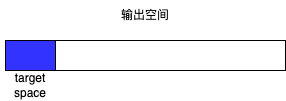
\includegraphics[width=0.4\textwidth]{./lecture2/lecture1-1.png} 
\end{figure}
输出空间很大,但是目标空间很小,这只能一个一个试nonce的值。这也是工作量证明(proof of work)。虽然挖矿很难,但是验证比较容易(difficult to solve, but easy to verify)。
\subsubsection*{2. 签名}
在比特币中开户其实就是创建一个\textbf{公私钥对}(public key, private key)。公钥相当于银行账户,私钥相当于密码。在进行交易时,用私钥进行签名,说明是本人进行的,发布交易时也要发送公钥,可供他人进行验证。

在这个过程中,产生公私钥对和签名时需要一个好的随机源(a good source of randomness)。
\subsection*{03-BTC-数据结构}
\subsubsection*{哈希指针}
hash pointer
\begin{figure}[H]
    \centering
    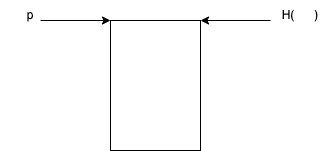
\includegraphics[width=0.4\textwidth]{./lecture3/img1.png} 
\end{figure}
Block chain is a linked list using hash pointer.
\begin{figure}[H]
    \centering
    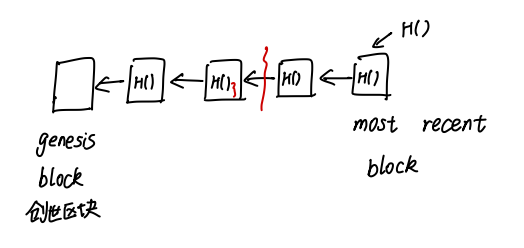
\includegraphics[width=0.5\textwidth]{./lecture3/img2.png} 
\end{figure}

实现\textbf{tamper-evident log},只要保存最后一个值,就知道前面有没有修改。
\subsubsection*{Merkle tree}
Merkle tree是用Hash指针代替普通指针的二叉树。
\begin{figure}[H]
    \centering
    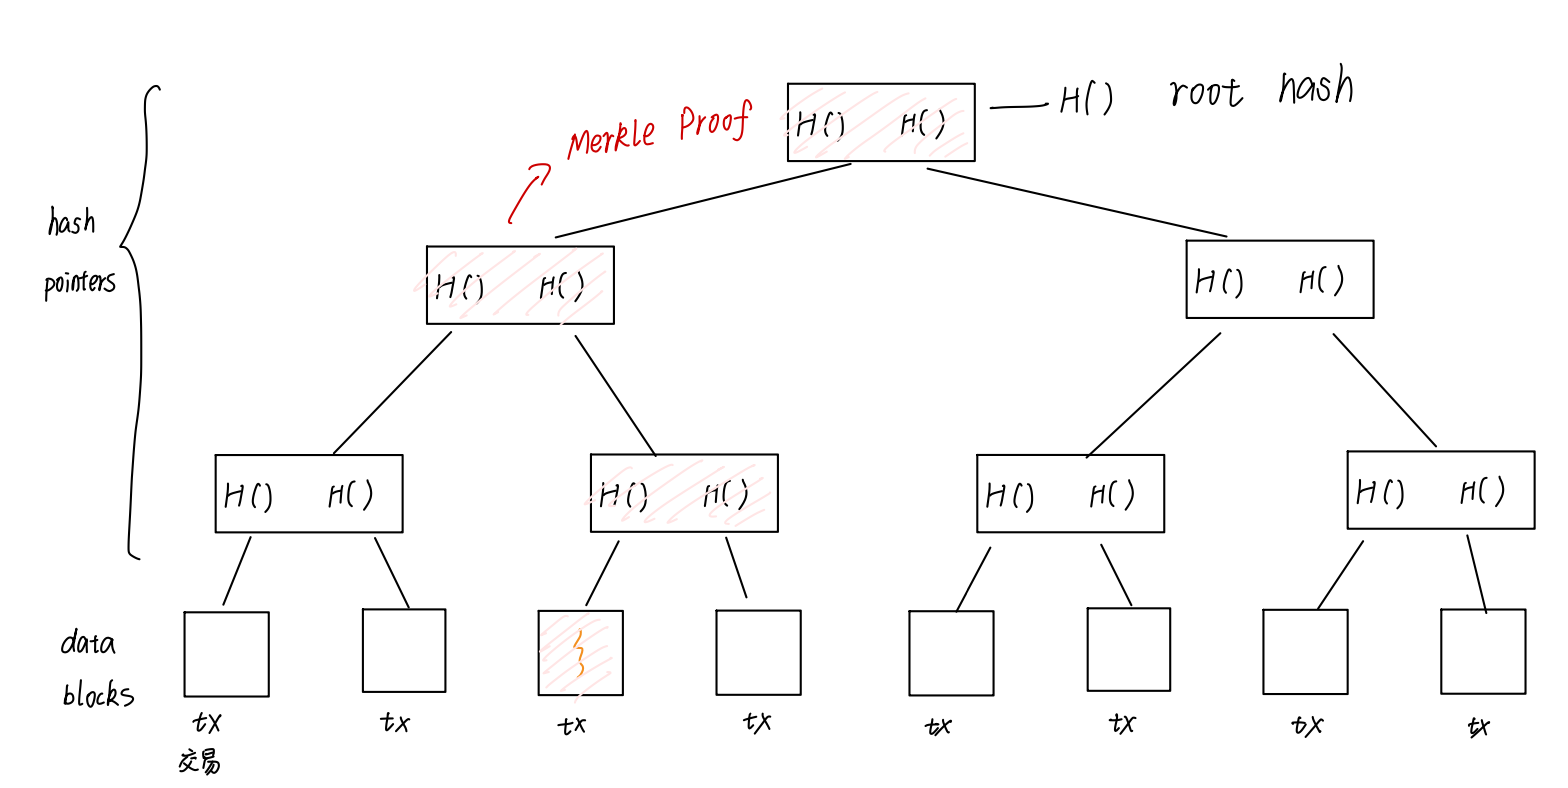
\includegraphics[width=1\textwidth]{./lecture3/img3.png} 
\end{figure}
\begin{itemize}
    \item block header (有root hash)
    \item block body (有交易列表)
\end{itemize}
Merkle tree的作用是可以提供Merkle proof,证明包含某种交易(\textbf{proof of membership / proof of inclusion}),是$O(\log(n))$的时间复杂度。但是如果证明某个交易不包含在Merkle tree中,如果进行所有叶子节点的遍历,时间复杂度是$O(n)$,这时可以考虑采用sorted Merkle tree,时间复杂度降为$O(\log(n))$。
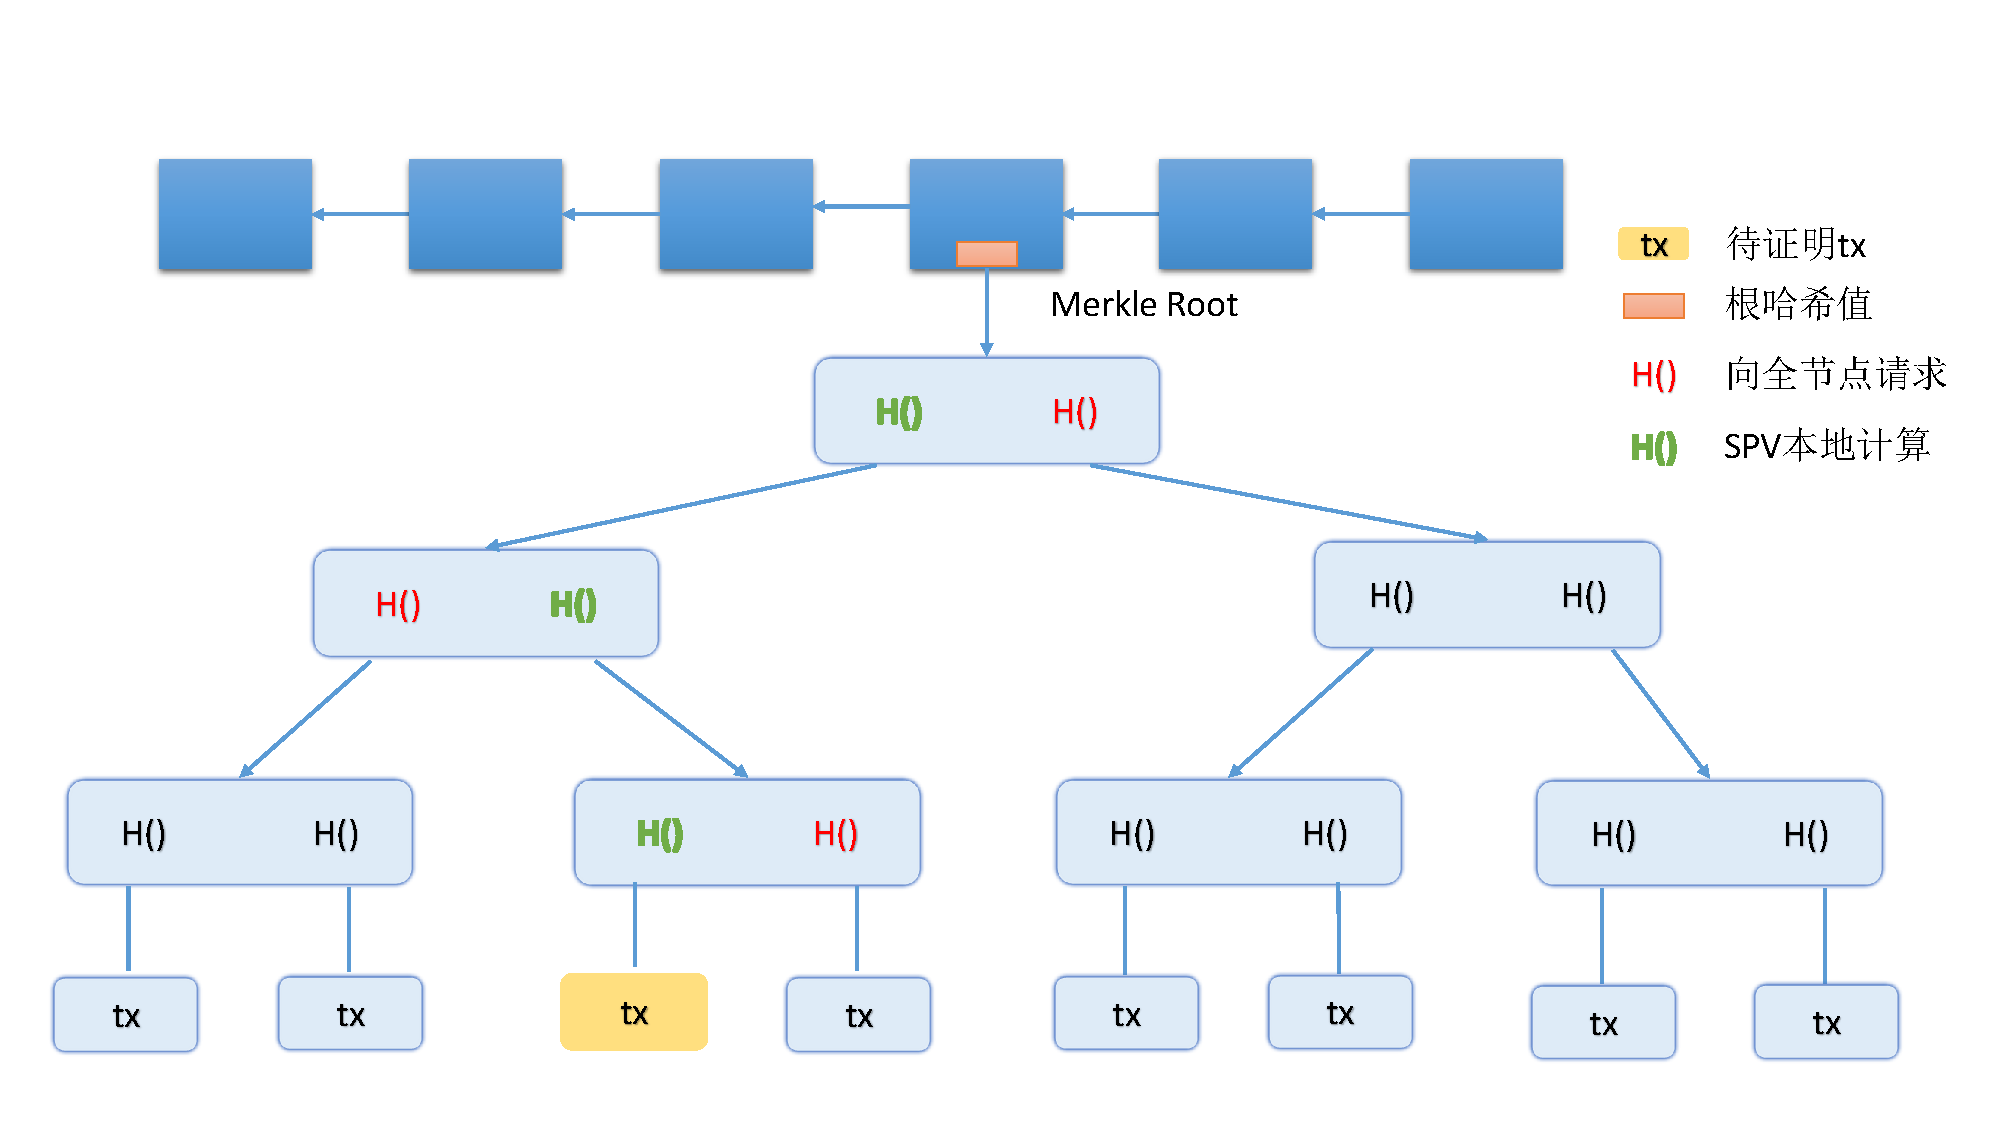
\includepdf[pages=1]{03-BTC.pdf} 
数据结构无环可以用hash pointer。如果有环会出现冲突。
\begin{figure}[H]
    \centering
    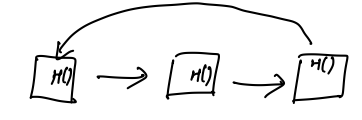
\includegraphics[width=0.5\textwidth]{./lecture3/img4.png} 
\end{figure}
\subsection*{04-BTC-协议}
如果中央银行要发售电子货币,每张纸币可以由中央银行签名。
\begin{figure}[H]
    \centering
    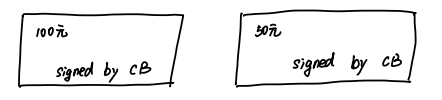
\includegraphics[width=0.5\textwidth]{./lecture4/img1.png} 
\end{figure}
这会出现双花攻击(double spending attack),因为这些电子货币其实就是代码,可以进行复制,我花出去一张100的,我可以复制很多张,继续花费。可以考虑维护一个数据库,给发行的每张货币一个编号,然后记录该货币属于谁,不过这样维护数据库就很麻烦了,而且也并不是去中心化的。
\begin{figure}[H]
    \centering
    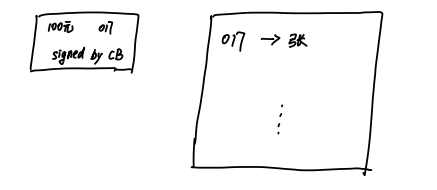
\includegraphics[width=0.5\textwidth]{./lecture4/img2.png} 
\end{figure}
比特币中的交易:
\begin{figure}[H]
    \centering
    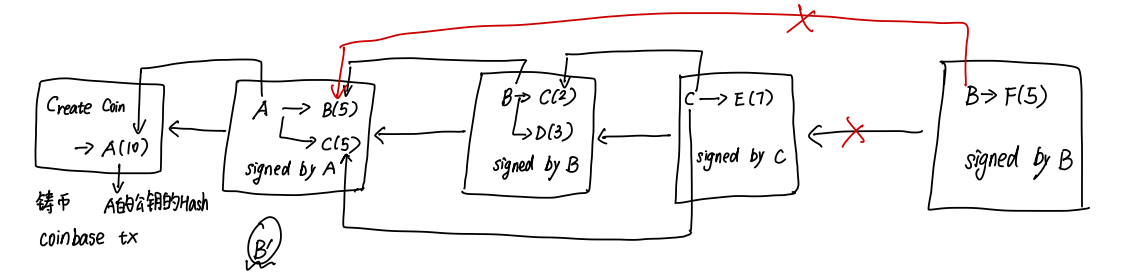
\includegraphics[width=1\textwidth]{./lecture4/img3.png} 
\end{figure}
A要给B转5个比特币,A需要知道B的地址。B也需要知道A的公钥,为了验证A的签名。在上图中,在交易时不仅要说明转账的地址,也要说明币的来源。在图中第二个区块中
\begin{itemize}
    \item 输入:币的来源、A的公钥
    \item 输出:B的公钥的哈希
\end{itemize}
这里就能避免双花,例如图中最后B想给F转5个比特币,可以看到B的5个比特已经花出去了,经过检查是不能再使用的。

脚本验证(Bitcoin Script):将输入与前一个输出拼接在一起,看是否能正确运行。
\begin{figure}[H]
    \centering
    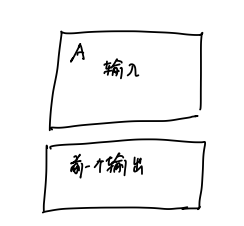
\includegraphics[width=0.3\textwidth]{./lecture4/img4.png} 
\end{figure}
每个块可以有很多交易,组织成Merkle tree。
\begin{figure}[H]
    \centering
    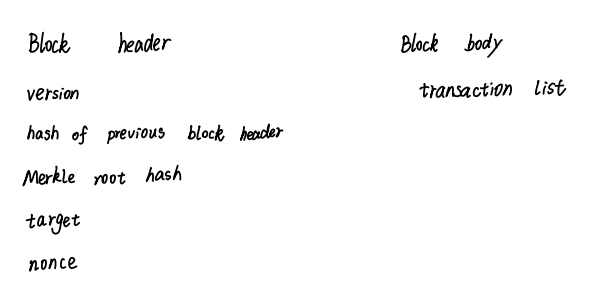
\includegraphics[width=0.7\textwidth]{./lecture4/img5.png} 
\end{figure}
\textbf{挖矿}:H(block header)$\le$target.区块链的另一种画法,因为其实哈希指针计算的是前一个block header中的哈希。
\begin{figure}[H]
    \centering
    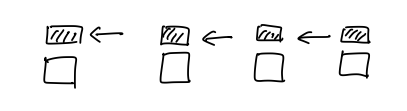
\includegraphics[width=0.6\textwidth]{./lecture4/img6.png} 
\end{figure}
\begin{itemize}
    \item full node: fully validating node,全节点记录所有信息
    \item light node: 轻节点
\end{itemize}

账本的内容要取得分布式的共识(distrubted consensus)。

FLP impossibilty result: 在异步系统中,网络传输时延没有上限,哪怕系统中只有一个成员是faulty,也没法达成共识。

CAP Theorem:任何一个分布式系统,以下3个性质中最多满足2个。
\begin{itemize}
    \item C: Consistency 一致性
    \item A: Availability
    \item P: Partition tolerance
\end{itemize}
Paxos协议满足Consistency性质。
\subsubsection*{Consensus in BitCoin}
重要的问题是:成员(membership)中谁拥有投票权。联盟链(hyperledger fabric)是只有加入链的成员有投票权。

女巫攻击(sybil attack):攻击方产生超过一半的用户。

如果节点能解决puzzle问题,可以获得记账权,有权利发布下一个节点。
\begin{figure}[H]
    \centering
    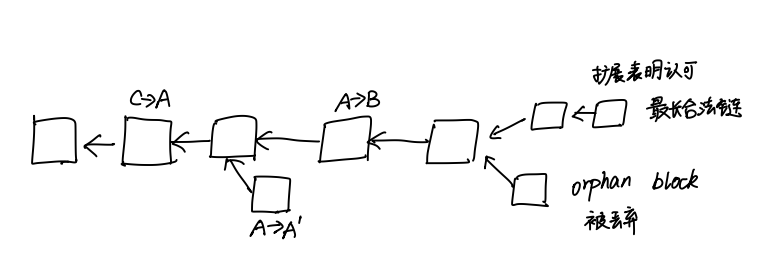
\includegraphics[width=1\textwidth]{./lecture4/img7.png} 
\end{figure}
longest vaild chain: 最长合法链

forking attack: 分叉攻击

block reward: 出块奖励

mining: 挖矿

miner: 矿工

coinbase transaction 是产生币的唯一方法。每隔21万个区块,区块奖励减半,50BTC$\rightarrow$25BTC$\rightarrow$12.5BTC.
\subsection*{05-BTC-实现}
比特币是基于交易记录的模式(\textbf{transaction-based ledger})。

\textbf{UTXO}: Unspent Transaction Output 还未花掉的交易的输出,为了检测双花,包含产生交易的哈希值以及在交易中的第几个。
\begin{figure}[H]
    \centering
    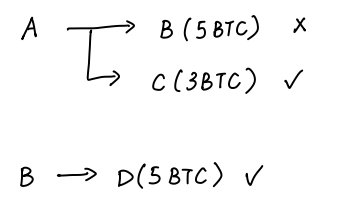
\includegraphics[width=0.4\textwidth]{./lecture5/img1.png} 
\end{figure}
B的5BTC已经花出去了,因此不在UTXO中。

total inputs = total outputs 所有输入=所有输出,但有时候不完全相等,例如所有输入为1BTC,所有输出为0.99BTC,这其中的差值是交易费(transaction fee)。比特币中大约每4年区块奖励会减半,因此到后期的奖励可能大部分来自于交易费。
$$
\frac{\text{21万区块}\times\text{10分钟}}{\text{60分钟}\times\text{24小时}\times\text{365天}} \approx \text{4年}
$$
还有一种模式是基于账户的模式(\textbf{account-based ledger}),例如以太坊。
\begin{figure}[H]
    \centering
    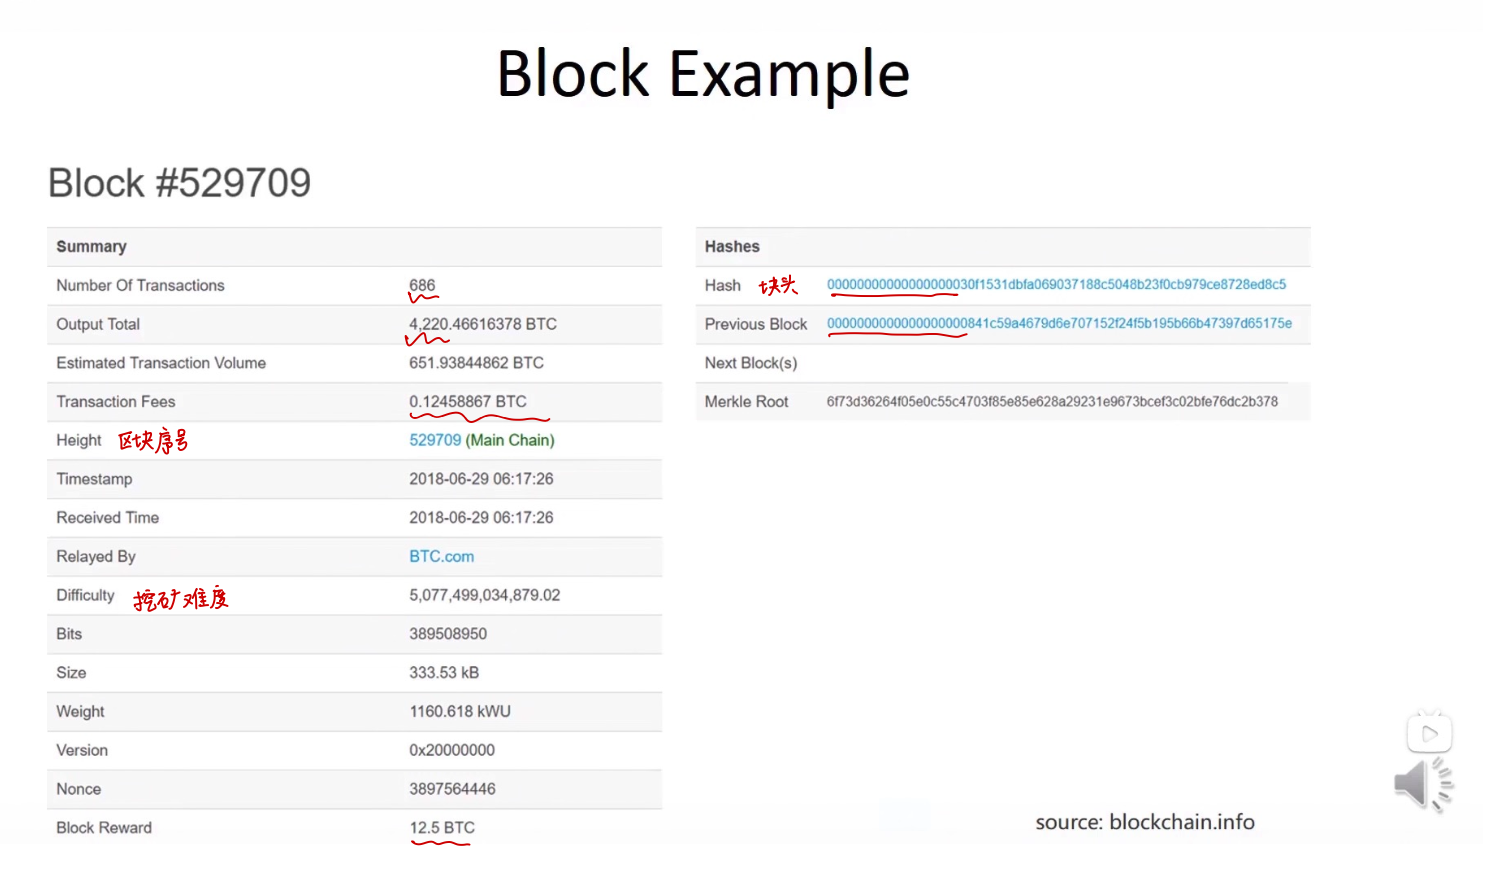
\includegraphics[width=1\textwidth]{./lecture5/img2.png} 
\end{figure}
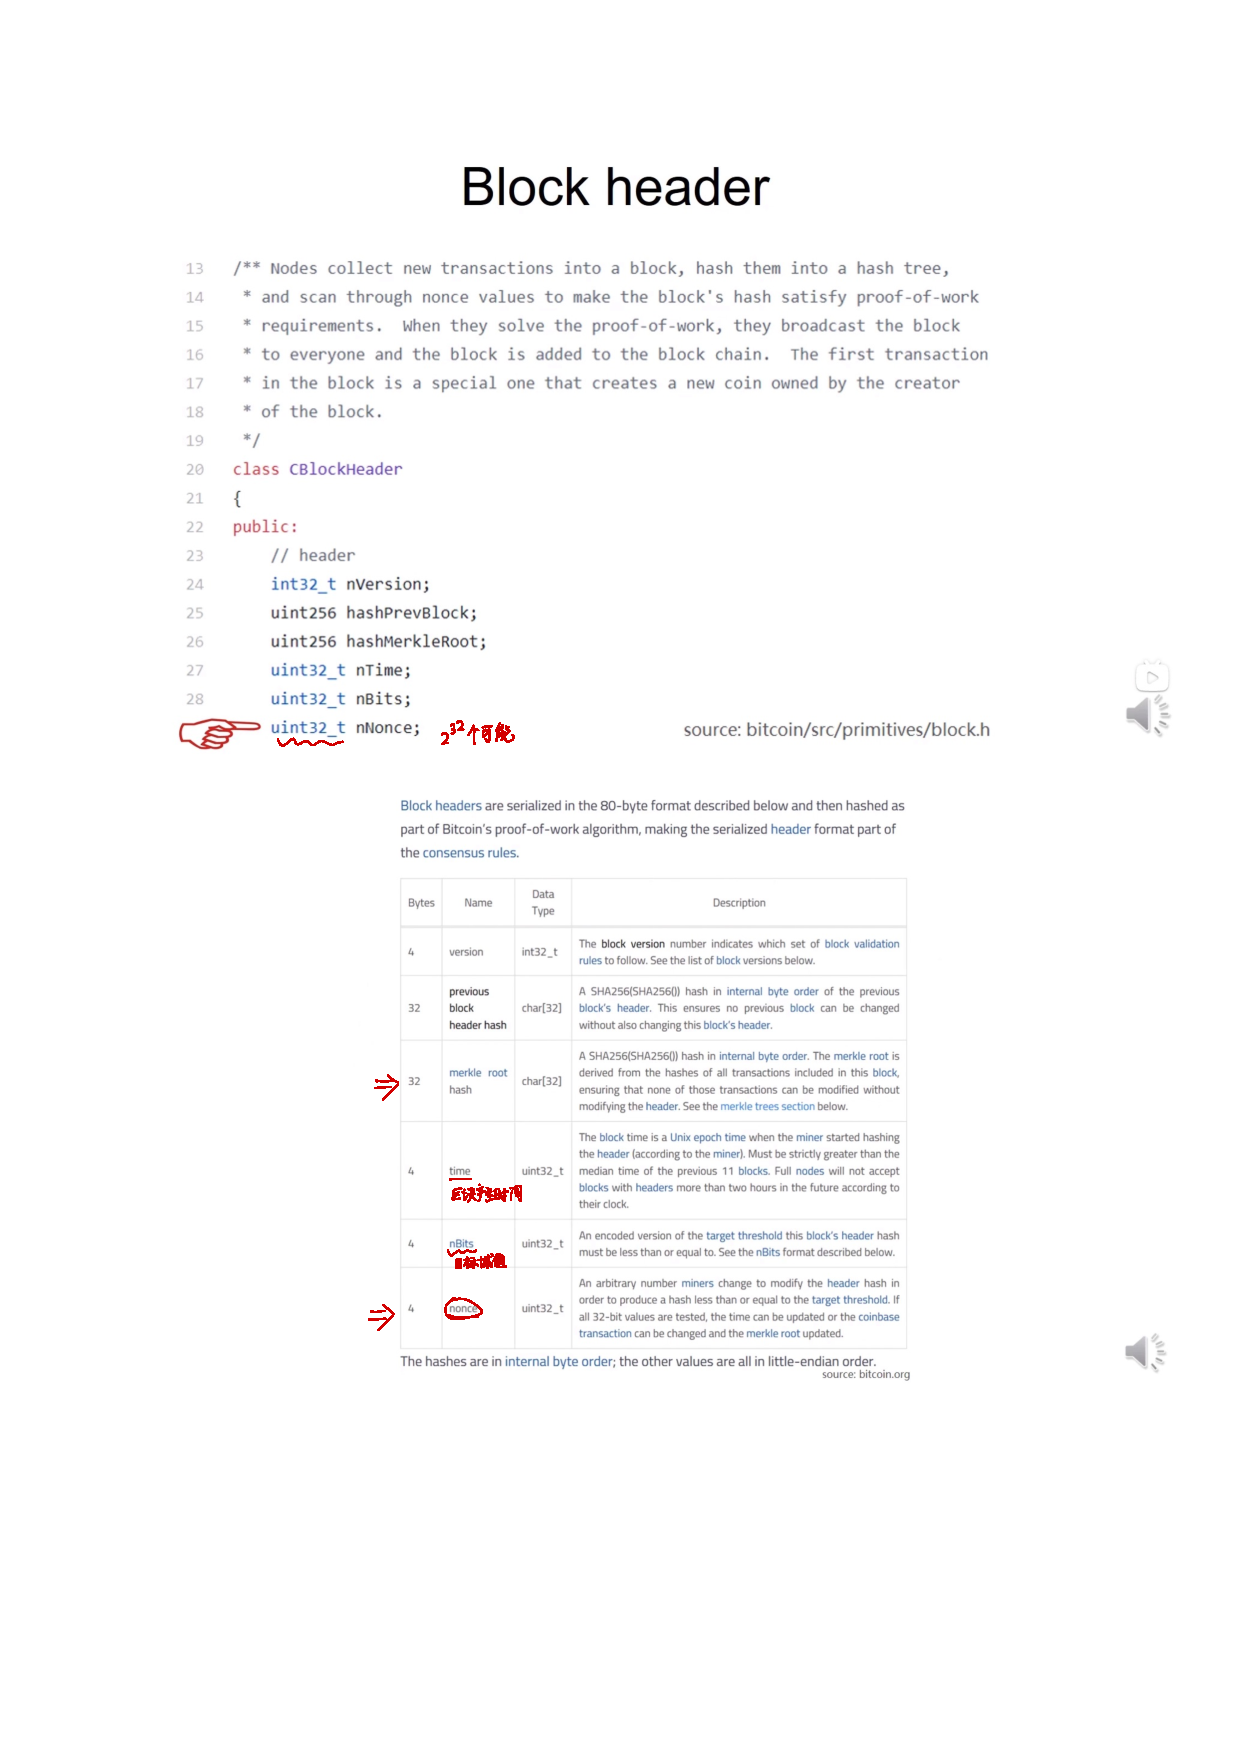
\includepdf[pages=-]{./lecture5/1.pdf} 
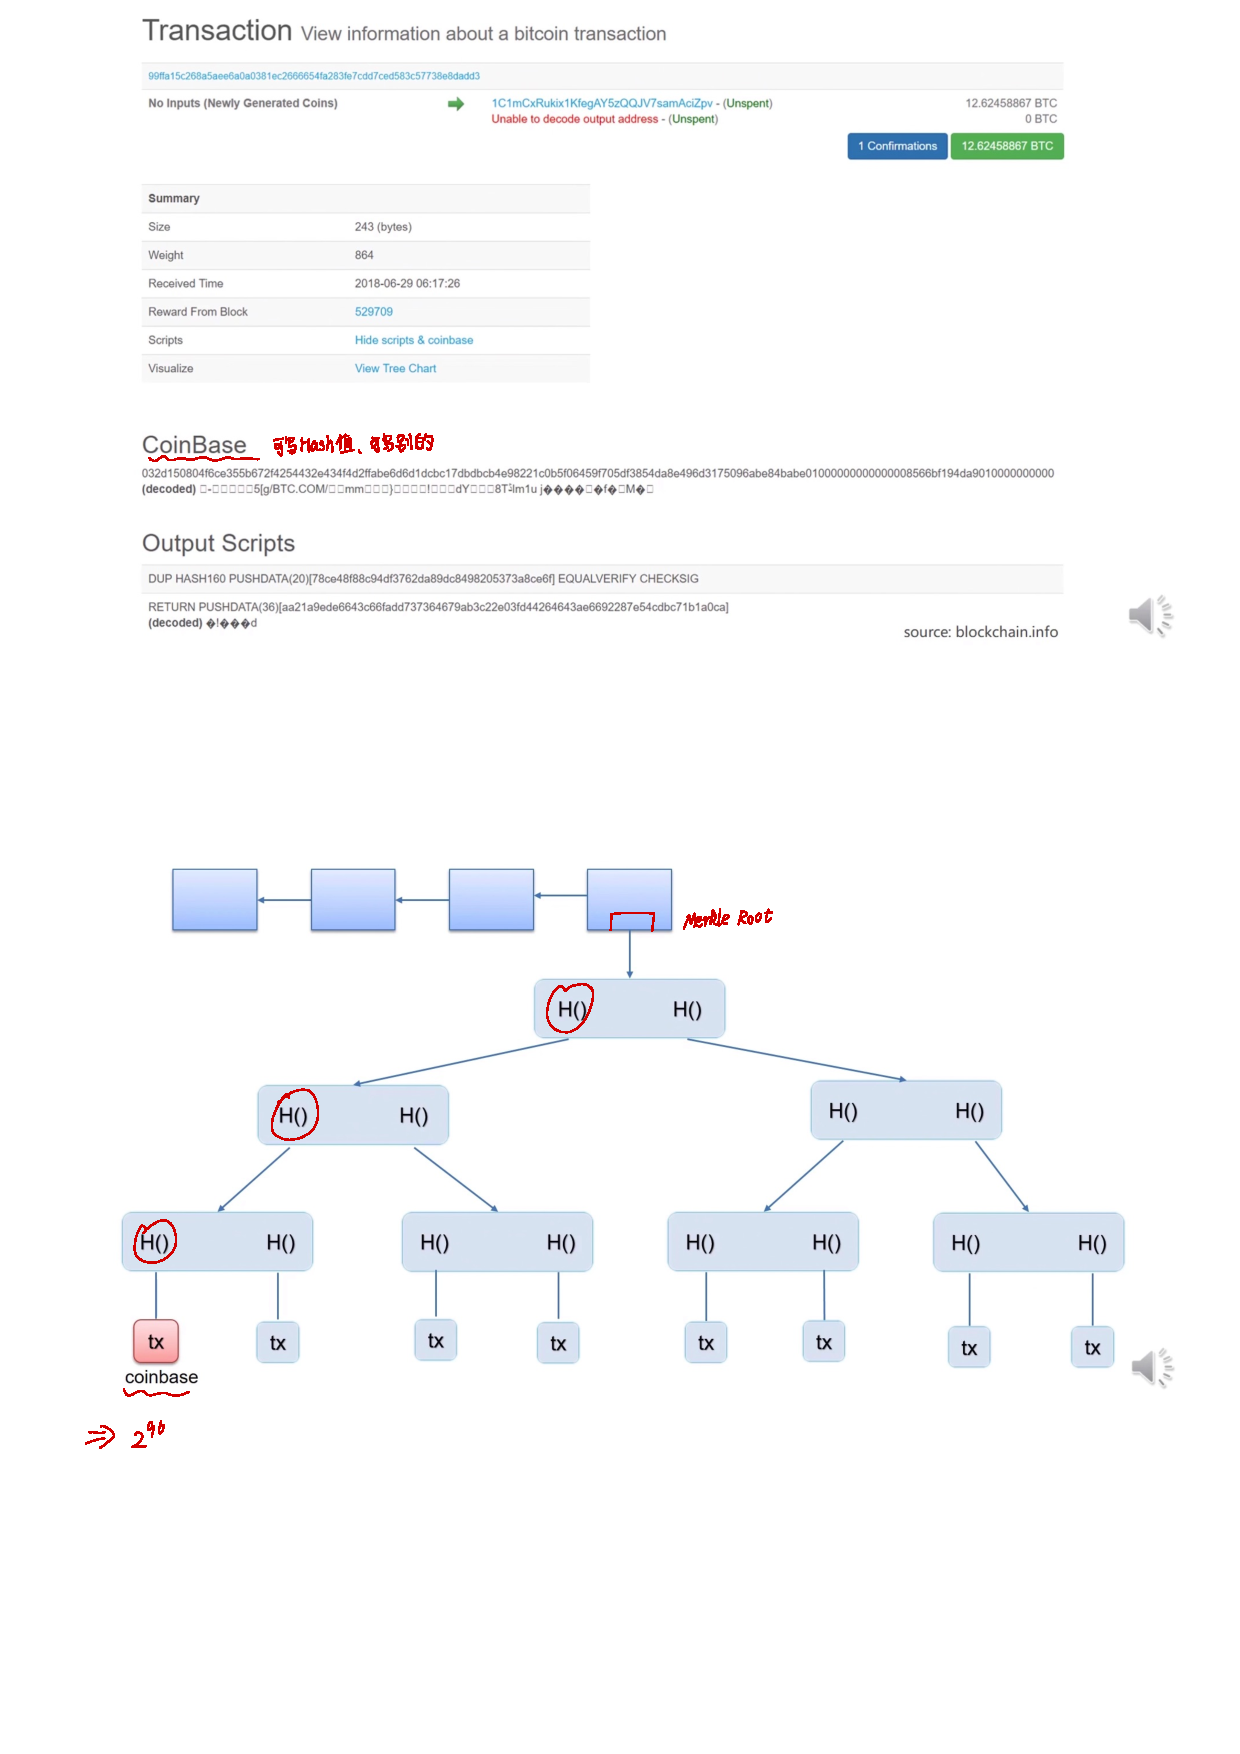
\includepdf[pages=-]{./lecture5/2.pdf} 
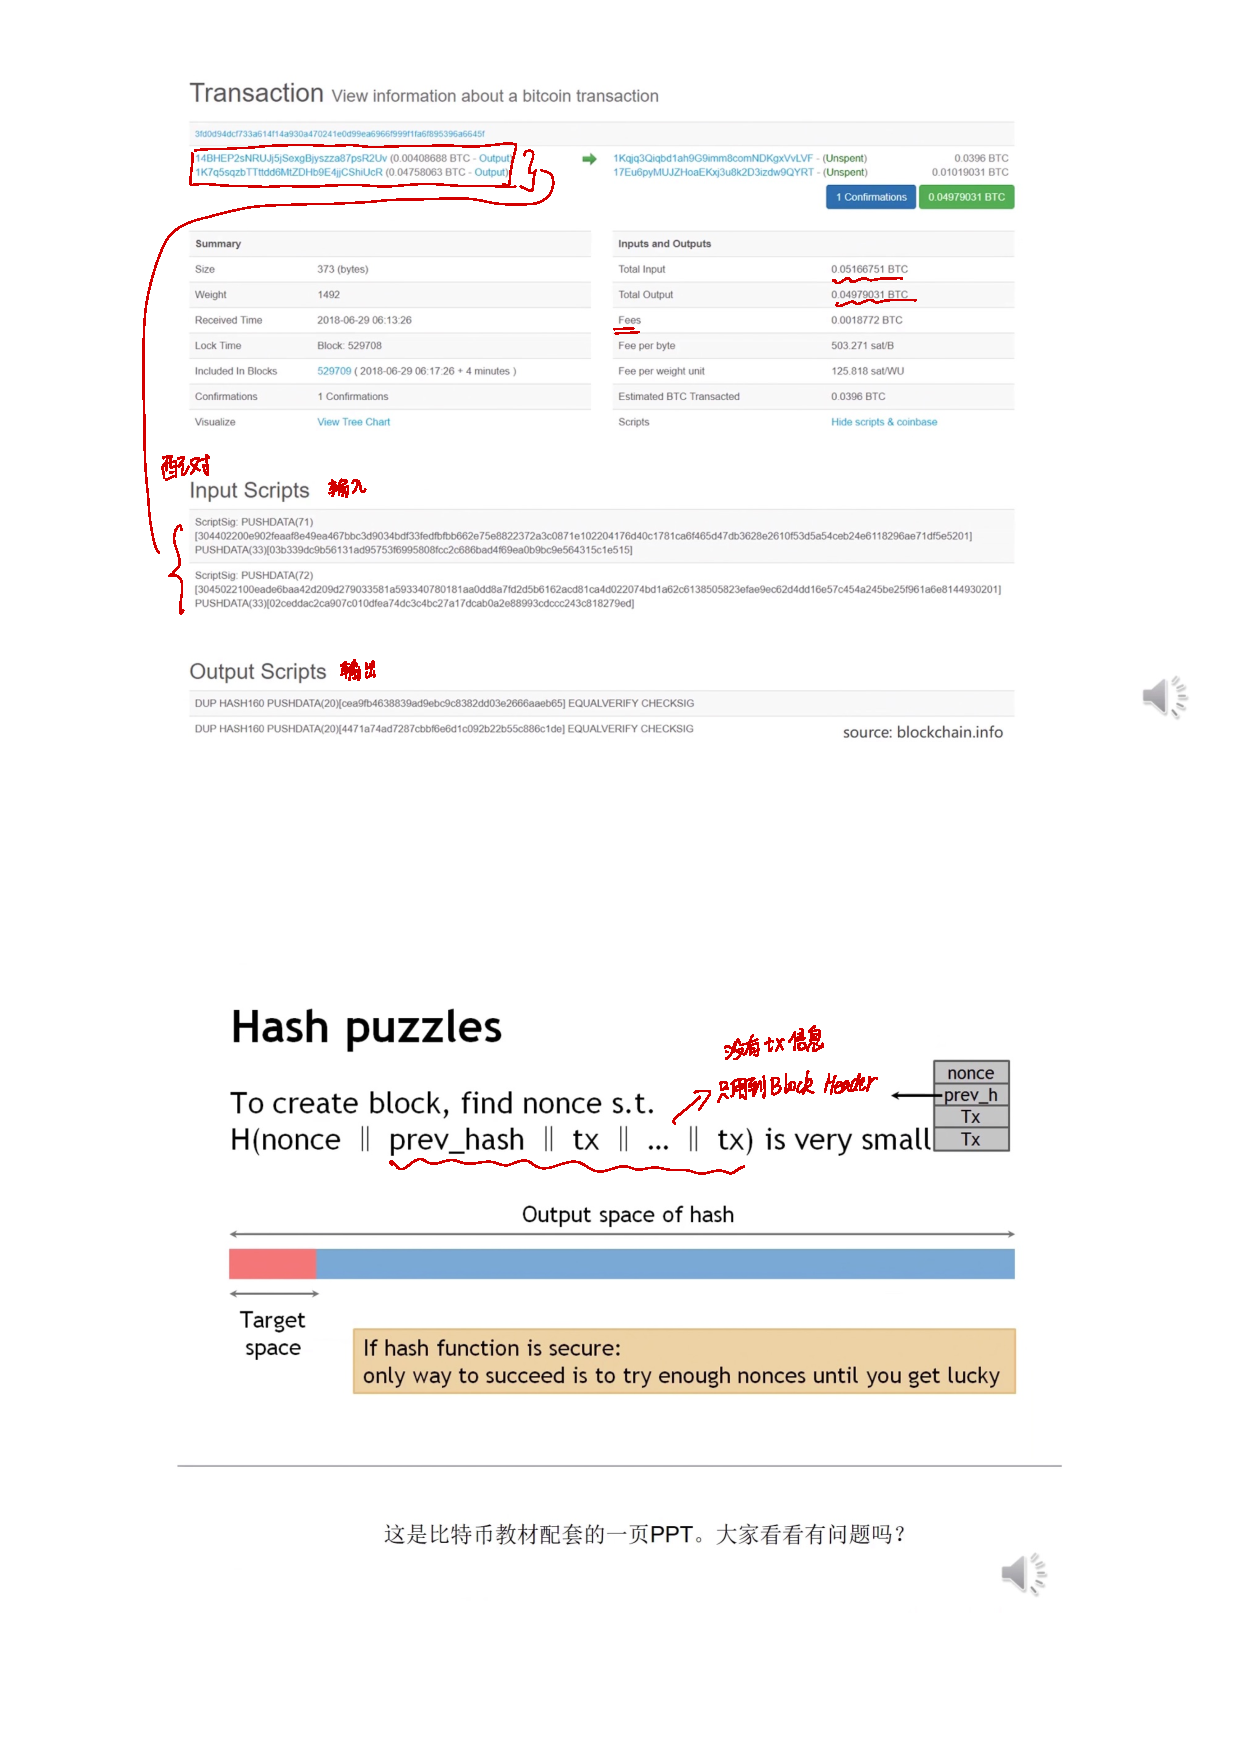
\includepdf[pages=-]{./lecture5/3.pdf} 
每次挖矿尝试看作是\textbf{Bernoulli trial}: a random experiment with binary outcome. Bernoulli process: a sequence of independent Bernoulli trials. Bernoulli process具有无记忆性(\textbf{memoryless})。大量的Bernolli process可用Poisson process近似。

出块时间服从指数分布(exponential distrubtion),也具有无记忆性。
\begin{figure}[H]
    \centering
    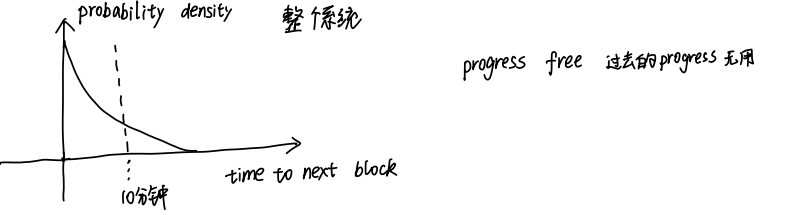
\includegraphics[width=1\textwidth]{./lecture5/img3.png} 
\end{figure}
产生比特币数量构成几何序列(geometric series)
\begin{figure}[H]
    \centering
    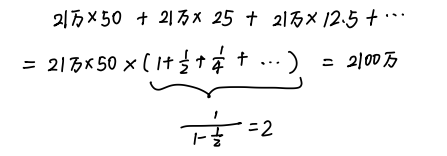
\includegraphics[width=0.5\textwidth]{./lecture5/img4.png} 
\end{figure}
BitCoin is secured by mining.
\begin{figure}[H]
    \centering
    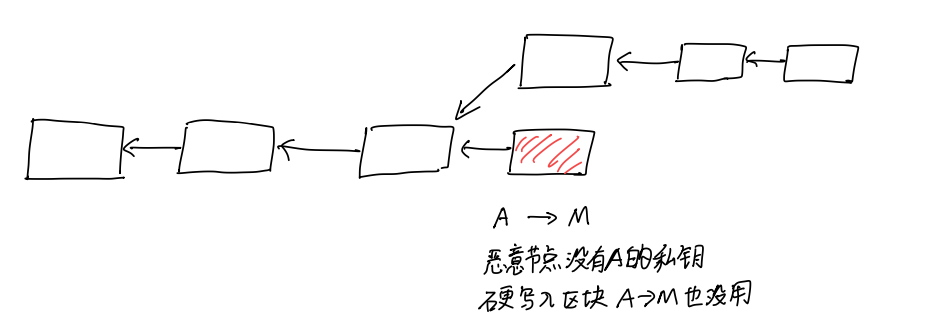
\includegraphics[width=1\textwidth]{./lecture5/img5.png} 
\end{figure}
double spending
\begin{figure}[H]
    \centering
    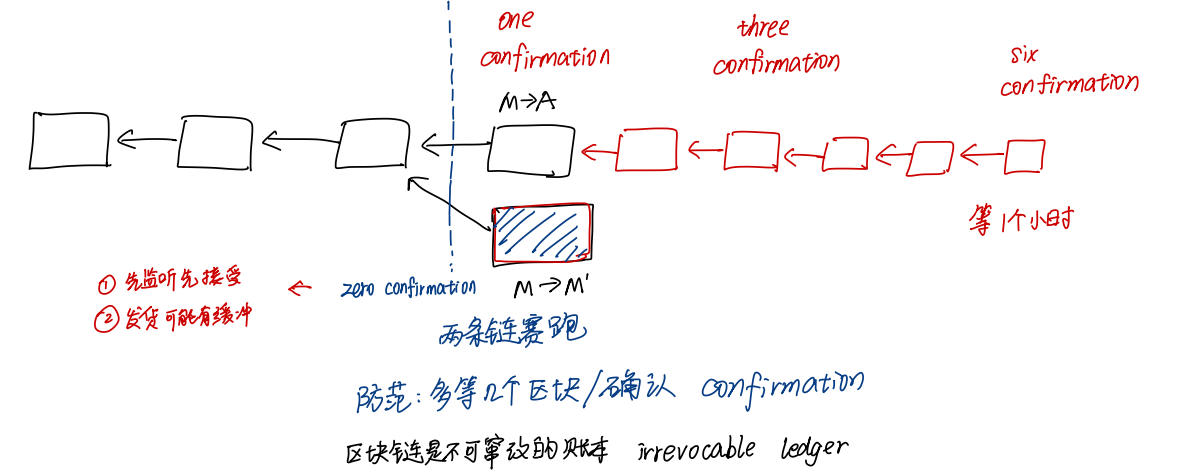
\includegraphics[width=1\textwidth]{./lecture5/img6.png} 
\end{figure}
selfish mining的分叉攻击,挖一长串,然后一下发布,这么做是有风险的。
\begin{figure}[H]
    \centering
    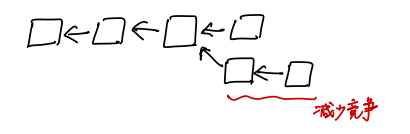
\includegraphics[width=0.5\textwidth]{./lecture5/img7.png} 
\end{figure}
\subsection*{06-BTC-网络}
上层是application layer: BitCoin Block chain.下层是network layer: P2P Overlay Network.比特币中各节点是对等的。

比特币网络设计原则:simple, robust(鲁棒), but not efficient.

flooding, 邻居节点的选取是随机的,因此两个节点可能地理上相隔很远,网络传输慢,并不是非常有效。全节点维护一个等待上链的集合,第一次听到转发,会在该集合中删除该交易,后续不转发。区块大小限制在1M。网络传播是尽力交付(best effort)。

\subsection*{07-BTC-挖矿难度}
H(block header) $\le$ target,挖矿难度
$$
\text{difficulty} = \frac{\text{difficulty\_1\_target}}{\text{target}}
$$
难度1,target更大。
\begin{figure}[H]
    \centering
    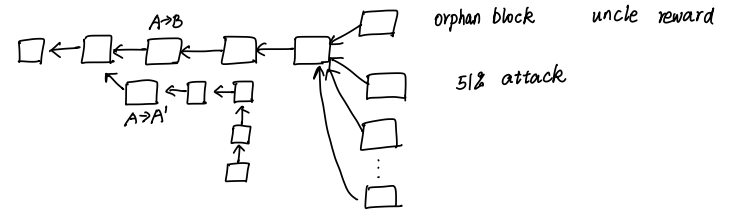
\includegraphics[width=1\textwidth]{./lecture7/img1.png} 
\end{figure}
出块时间越短,出现分叉的可能更多。

以太坊协议 ghost,平均出块时间需要保持稳定。

调整挖矿难度:
$$
\text{target} = \text{target} \times \frac{\text{actual time}}{\text{expected time}}
$$
其中,acutual time是最近挖出2016区块的时间,期望时间expected time = $2016 \times 10$,理想的挖出2016个区块的时间是两周。难度最大增长4倍,最小也是缩小4倍。
\subsection*{08-BTC-挖矿}
\subsection*{09-BTC-比特币脚本}
\subsection*{10-BTC-分叉}
\end{document}
